% \documentclass[mat2, tisk]{fmfdelo}
% \documentclass[fin2, tisk]{fmfdelo}
\documentclass[isrm2, tisk]{fmfdelo}
% \documentclass[ped, tisk]{fmfdelo}
% Če pobrišete možnost tisk, bodo povezave obarvane,
% na začetku pa ne bo praznih strani po naslovu, …

%%%%%%%%%%%%%%%%%%%%%%%%%%%%%%%%%%%%%%%%%%%%%%%%%%%%%%%%%%%%%%%%%%%%%%%%%%%%%%%
% METAPODATKI
%%%%%%%%%%%%%%%%%%%%%%%%%%%%%%%%%%%%%%%%%%%%%%%%%%%%%%%%%%%%%%%%%%%%%%%%%%%%%%%

% - vaše ime
\avtor{Tim Kalan}

% - naslov dela v slovenščini
\naslov{Večstranski podpisi}

% - naslov dela v angleščini
\title{Multisignatures}

% - ime mentorja/mentorice s polnim nazivom:
%   - doc.~dr.~Ime Priimek
%   - izr.~prof.~dr.~Ime Priimek
%   - prof.~dr.~Ime Priimek
%   za druge variante uporabite ustrezne ukaze
\mentor{doc.~dr.~Tilen Marc}
% \somentor{...}
% \mentorica{...}
% \somentorica{...}
% \mentorja{...}{...}
% \somentorja{...}{...}
% \mentorici{...}{...}
% \somentorici{...}{...}

% - leto magisterija
\letnica{2024}

% - povzetek v slovenščini
%   V povzetku na kratko opišite vsebinske rezultate dela. Sem ne sodi razlaga
%   organizacije dela, torej v katerem razdelku je kaj, pač pa le opis vsebine.
\povzetek{Tukaj napišemo povzetek vsebine. Sem sodi razlaga vsebine in ne opis tega, kako je delo organizirano.}

% - povzetek v angleščini
\abstract{An abstract of the work is written here. This includes a short description of
the content and not the structure of your work.}

% - klasifikacijske oznake, ločene z vejicami
%   Oznake, ki opisujejo področje dela, so dostopne na strani https://www.ams.org/msc/
\klasifikacija{94A60, 11T71}

% - ključne besede, ki nastopajo v delu, ločene s \sep
\kljucnebesede{digitalni podpis\sep kriptografija}

% - angleški prevod ključnih besed
\keywords{digital signature\sep cryptography} % angleški prevod ključnih besed

% - neobvezna zahvala
\zahvala{
  Neobvezno.
  Zahvaljujem se \dots
}

% - program dela, ki ga napiše mentor z osnovno literaturo
\programdela{
  Mentor naj napiše program dela skupaj z osnovno literaturo.
}

\osnovnaliteratura{
% Literatura mora biti tukaj posebej samostojno navedena (po pomembnosti) in ne
% le citirana. V tem razdelku literature ne oštevilčimo po svoje, ampak uporabljamo
% ukaz \vnosliterature, v katerega vpišemo citat
  \vnosliterature{micali2001asm}
  % \vnosliterature{gurtin1982introduction}
  % \vnosliterature{zienkiewicz2000finite}
  % \vnosliterature{STtemplate}
}

% - ime datoteke z viri (vključno s končnico .bib), če uporabljate BibTeX
\literatura{literatura.bib}

%%%%%%%%%%%%%%%%%%%%%%%%%%%%%%%%%%%%%%%%%%%%%%%%%%%%%%%%%%%%%%%%%%%%%%%%%%%%%%%
% DODATNE DEFINICIJE
%%%%%%%%%%%%%%%%%%%%%%%%%%%%%%%%%%%%%%%%%%%%%%%%%%%%%%%%%%%%%%%%%%%%%%%%%%%%%%%

% naložite dodatne pakete, ki jih potrebujete
\usepackage{units}        % fizikalne enote kot \unit[12]{kg} s polovico nedeljivega presledka, glej primer v kodi
\usepackage{graphicx}     % za slike
% \usepackage{tikz}
% VEČ ZANIMIVIH PAKETOV
% \usepackage{array}      % več možnosti za tabele
% \usepackage[list=true,listformat=simple]{subcaption}  % več kot ena slika na figure, omogoči slika 1a, slika 1b
% \usepackage[all]{xy}    % diagrami
% \usepackage{doi}        % za clickable DOI entrye v bibliografiji
% \usepackage{enumerate}     % več možnosti za sezname

% Za barvanje source kode
% \usepackage{minted}
% \renewcommand\listingscaption{Program}

% Za pisanje psevdokode
% \usepackage{algpseudocode}  % za psevdokodo
% \usepackage{algorithm}
% \floatname{algorithm}{Algoritem}
% \renewcommand{\listalgorithmname}{Kazalo algoritmov}

% deklarirajte vse matematične operatorje, da jih bo LaTeX pravilno stavil
% \DeclareMathOperator{\...}{...}

% vstavite svoje definicije ...
\newcommand{\R}{\mathbb R}
\newcommand{\N}{\mathbb N}
\newcommand{\Z}{\mathbb Z}
% Lahko se zgodi, da je ukaz \C definiral že paket hyperref,
% zato dobite napako: Command \C already defined.
% V tem primeru namesto ukaza \newcommand uporabite \renewcommand
\newcommand{\C}{\mathbb C}
\newcommand{\Q}{\mathbb Q}

%%%%%%%%%%%%%%%%%%%%%%%%%%%%%%%%%%%%%%%%%%%%%%%%%%%%%%%%%%%%%%%%%%%%%%%%%%%%%%%
% ZAČETEK VSEBINE
%%%%%%%%%%%%%%%%%%%%%%%%%%%%%%%%%%%%%%%%%%%%%%%%%%%%%%%%%%%%%%%%%%%%%%%%%%%%%%%

\begin{document}

\section{Uvod}
% Napišite kratek zgodovinski in matematični uvod.  Pojasnite motivacijo za problem, kje
% nastopa, kje vse je bil obravnavan. Na koncu opišite tudi organizacijo dela -- kaj je v
% katerem razdelku.
Odkar se je na svetu pojavil koncept (ročnega) podpisa, je večina primerov uporabe temeljila na
pridobivanju podpisov več deležnikov. Odličen primer je npr.\ Deklaracija neodvisnosti Združenih 
držav Amerike. SLIKA?. 

V prejšnjem stoletju je vzpon računalnika in napredek v kriptografiji privedel do \textit{digitalnih
podpisov}. Ti odlično nadomeščajo ročni podpis, prav tako omogočajo, da se skupina podpiše tako, 
da vsak član poda svoj podpis. Vendar tu lahko z malo matematike poskrbimo, da se skupina lahko 
podpiše tako, da vsi člani skupaj oddajo en sam podpis, ki priča o podpisu celotne skupine. Tako 
razbremenimo preverjalca podpisov, kar je ključno v sistemih, kjer je računska moč omejena ali 
pa draga (npr.\ pri tehnologiji veriženja blokov).

\section{Kriptografske osnove}
Preden si lahko pogledamo točno kako lahko skupina generira en sam podpis besedila, si moramo 
pogledati nekaj kriptografskih osnov. Bolj komplicirane stvari bodo opisane sproti, ideja tega 
poglavja je predstaviti stvari, ki so predpogoj za branje kakršnegakoli kriptografskega 
besedila.

\subsection{Aritmetika v $\Z_p^*$}
V kriptografiji imamo pogosto opravka z multiplikativnimi grupami, najenostavnejša med njimi (in 
tudi tradicionalno največ uporabljena) je \textit{multiplikativna grupa naravnih števil modulo $p$} 
$\Z_p^*$. Njeni elementi so števila v $\{0, 1, \dots, p - 1\}$, ki so tuja številu $p$. V posebnem 
primeru, ko je $p$ praštevilo, so to torej števila \{1, 2, \dots, p - 1\} in je red grupe 
$\text{ord}(\Z_p^*) = |\Z_p^*| = p - 1$. Operacija v tej grupi je, kot ime že nakazuje, množenje 
modulo $p$.

Spomnimo se, da je red elementa $g$ najmanjše naravno število $q$, da velja $g^q \equiv 1 \pmod p$, 
kjer je $1$ enota za množenje. V primeru, da je $p$ praševilo, je grupa grupa $\Z_p^*$ \textit{ciklična}, 
kar pomeni, da v njej obstaja element $g$, katerega red je enak redu grupe, torej $\text{ord}(g) = p - 1$.
V tem primeru se $g$ imenuje \textit{generator}.

\begin{primer}[Grupa $\Z_{11}^*$]
Ker je $11$ praštevilo, v grupi $\Z_{11}^*$ obstaja generator, oz.\ je grupa ciklična z redom $10 = 
11 - 1$. Z zaporednim računanjem potenc lahko vidimo, da je $\text{ord}(2) = 10$, torej je $2$ 
generator.

\begin{minipage}{0.45\textwidth}
    \begin{align*}
        2^1 &\equiv 2 \pmod{11} \\
        2^2 &\equiv 4 \pmod{11} \\
        2^3 &\equiv 8 \pmod{11} \\
        2^4 &\equiv 5 \pmod{11} \\
        2^5 &\equiv 10 \pmod{11} 
    \end{align*}
\end{minipage}
\begin{minipage}{0.45\textwidth}
    \begin{align*}
        2^6 &\equiv 9 \pmod{11} \\
        2^7 &\equiv 7 \pmod{11} \\
        2^8 &\equiv 3 \pmod{11} \\
        2^9 &\equiv 6 \pmod{11} \\
        2^{10} &\equiv 1 \pmod{11} 
    \end{align*}
\end{minipage}

\end{primer}

\begin{opomba}
    Spomnimo se \textit{kongruence}: $a \equiv b \pmod m \iff m \text{ }|\text{ } a - b$.
\end{opomba}

\subsection{Zgoščevalne funkcije}
V grobem so (kriptografske) \textit{zgoščevalne funkcije} funkcije, ki prejmejo poljubno dolg binarni 
niz (ki lahko predstalja besede, številke, celotne dokumente, \dots), vrnejo pa binarni niz, ki ima 
vnaprej določeno dolžino. Tem rezultatom pravimo \textit{zgostitve}. Namen zgoščevalnih funkcij je 
za dokument ustvariti unikaten niz, ki zelo verjetno identiificira dokument. V grobem si od zgoščevalnih 
funkcij želimo naslednje lastnosti:
\begin{itemize}
    \item \textbf{Določenost} pomeni, da bo zgoščevanje enakih nizov vedno privedlo do enake 
        zgostitve. 
    \item \textbf{Učinkovitost} pomeni, da lahko računalnik izračuna poljubno zgostitev v doglednem 
        času. Izračun zgostitve mora biti računsko učinkovit.
    \item \textbf{Enosmernost} pomeni, da iz predložene zgostitve zelo težko ugotovimo, kater niz 
        je funkcija prejela kot vhod. Tej lastnosti pravimo tudi \textit{odpornost na prasliko}.
    \item \textbf{Odpornost na drugo prasliko} pomeni, da če poznamo niz in njegovo zgostitev, 
        je zelo težko najdemo drug niz z enako zgostitvijo.
    \item \textbf{Skoraj brez trčenj} pomeni, da je verjetnost, da imata dva izraza enako zgostitev,
        majhna. Želimo tudi, da je zelo težko najti dva niza z enako zgostitvijo.
    \item \textbf{Učinek plazu} pomeni, da majhna sprememba v vhodnem nizu povzroči veliko spremembo 
        v zgostitvi.
\end{itemize}

\begin{definicija} 
\label{def:hash}
    \textbf{Kriptografska zgoščevalna funkcija} $H: \{0, 1\}^* \rightarrow \{0, 1\}^n$ je funkcija, 
    ki slika binarne nize $m$ poljubne dolžine v njihove \textbf{zgostitve} $H(m)$, tj.\ binarne nize 
    vnaprej določene dolžine $n$. Zadoščati mora naslednjim lastnostim:
    \begin{itemize}
        \item (določenost) $\forall m: ((h_1 = H(m) \wedge h_2 = H(m)) \implies h_1 = h_2)$.
        \item (učinkovitost) Izračun funkcije $H$ mora biti računsko učinkovit.
        \item (odpornost na prasliko) Če poznamo zgostitev $h$ je računsko neizvedljivo najti 
            niz $m$, da velja $h = H(m)$.
        \item (odpornost na drugo prasliko) Če poznamo niz $m_1$ je računsko neizvedljivo najti 
            zgostitev $m_2$, da velja $H(m_1) = H(m_2)$.
        \item (odpornost na trčenja) Računsko neizvedljivo je najti dva niza $m_1$ in $m_2$, 
            da velja $H(m_1) = H(m_2)$.
        \item (učinek plazu) Vsaka sprememba vhoda povzroči, veliko spremembo v zgostitvi. 
            Vsak bit zgostitve se spremeni z verjetnostjo vsaj $1/2$.
    \end{itemize}
\end{definicija}

\begin{primer}
    Ena izmed najbolj znanih zgostitvenih funkcij je \texttt{SHA-256}. Njeno ime pomeni \textit{Secure 
    Hash Algorithm} (slov.\ varen zgostitveni algoritem), $256$ pa predstavlja dolžino zgostitve. 
    Pogostokrat to ime zasledimo pri nameščanju programske opreme, služi kot avtentikator, da smo res 
    naložili pravo stvar.

    Za primer si lahko ogledamo zgostitvi dveh podobnih nizov, \textit{Ljubljana} in \textit{Ljubljena}. 
    Kljub podobnosti bomo videli, da sta rezultata popolnoma drugačna, kar si tudi želimo pri zgostitvenih 
    funkcijah.
    \begin{verbatim}
    SHA-256(Ljubljana) =
    b7f147d8b4a6703a951336654355071f9752385f85d0860379e99b484aee7a82

    SHA-256(Ljubljena) =
    995d2d8ffb40e1838219e65dd2c665701ba34a90e11f7195a4b791838b6787fe
    \end{verbatim}
    Za preglednost nismo prevajali besed v binarne nize, to bi storili npr.\ z \texttt{ASCII} ali \texttt{UTF-8}
    tabelo. Prav tako smo rezultat napisali v šestnajstiškem sistemu, saj je tako krajši.
\end{primer}

\subsection{Kriptografija javnega ključa}
Prve šifre, ki smo jih uporabljaji ljudje, so bile \textit{simetrične}, kar pomeni, da sta osebi 
za komunikacijo obe morali poznati skriven \textit{ključ}, ki je definiral, kako je bila šifra 
ustvarjena. 

\begin{primer}[Cezarjeva šifra]
    Ena najbolj znanih šifer, ki izvira iz Antičnega Rima, je \textit{Cezrjeva šifra}. Njen ključ 
    je število, ki je krajše od dolžine naše abecede, v Cezarjevem primeru je bilo to število $3$.
    Šifra potem deluje tako, da vsako črko zamaknemo za toliko mest v abecedi, kolikor definira 
    ključ. Npr.\ za slovensko abecedo, bi šifra zamaknila črke:
    \begin{verbatim}
        A B C Č D E F G H I J K L M N O P R S Š T U V Z Ž
        Č D E F G H I J K L M N O P R S Š T U V Z Ž A B C
    \end{verbatim}
    To bi izraz \texttt{JAVNI KLJUČ} preslikalo v \texttt{MČARL NOMŽF}. Cezarjeva šifra se imenuje 
    tudi \textit{zamična šifra}.
\end{primer}

V prejšnjem stoletju pa se je pojavila alternativa, imenovana \textit{asimetrična kriptografija}, oz.\
\textit{kriptografija javnega ključa}. Glavna prednost te je, da osebi za komunikacijo ne rabita 
poznati enakega skrivnega ključa, vendar ima vsak od njiju par ključev, ki ju imenujemo \textit{javni 
ključ} (angl.\ \textit{public key}) in \textit{zasebni ključ} (angl.\ \textit{secret/private key})in 
označimo kot par $(\text{pk}, \text{sk})$. Vsaka oseba objavi svoj javni ključ in poskrbi, da nihče 
ne izve, kaj je njen zasebni ključ. 

Šifriranje potem poteka tako, da pridobimo javni ključ od osebe, s katero želi komunicirati, ga uporabi
za šifriranje in objavi šifrirano sporočilo. Lastnik ustreznega zasebnega ključa (vsakemu javnemu pripada 
natanko en zasebni) potem pridobi šifrirano sporočilo in ga z zasebnim ključem odšifrira. Kriptosistemi 
delujejo na način, da lahko sporočilo, šifrirano z javnim ključem odšifrira samo ustrezen zasebni ključ. 
Tako zagotovimo varno komunikacijo. 

\begin{primer}[RSA]
    En prvih algoritmov javnega ključa, ki se uporablja še danes, je \textit{RSA}. Njegova varnost izhaja 
    iz (domnevne) težavnosti problema iskanja prafaktorjev. Svoj ključ definiramo tako, da si izberemo dve 
    (zelo veliki) praštevili $p$ in $q$, ter ju zmnožimo v $n = pq$. Za primer vzemimo $p = 23$ in 
    $q = 17$. $n$ je potem enak $391$. Izbrati si moramo še eksponent $e$, vzemimo npr. $e = 3$. Naš 
    javni ključ je potem par 
    $$ 
    (n, e) = (391, 3).
    $$
    Postopek šifriranja poteka tako, da oseba, s katero komuniciramo, izbere sporočilo $m$, npr.\ 
    $m = 10$, pridobi naš javni ključ, in izračuna šifro $c$ kot
    $$   
    c = m^e \bmod{n} = 10^3 \bmod{n} = 218.
    $$
    Dogovoriti se moramo še o zasebnem ključu. Za to bomo potrebovali eksponent za odšifriranje $d$,
    tako da bo veljalo 
    $$
    (m^e)^d \equiv 1 \pmod{\varphi(n)},
    $$ 
    kjer $\varphi$ označuje Eulerjevo funkcijo fi. Iščemo torej multiplikativni inverz eksponenta 
    $e$, modulo $\varphi(n)$. V našem primeru je to $d = 235$. Zasebni ključ je potem 
    $$ 
    (p, q, d) = (23, 17, 235). 
    $$
    Iz zasebnega ključa torej lahko kadarkoli izračunamo javnega, saj enostavno zmnožimo $p$ in $q$ 
    ter izračunamo inverz, v splošnem pa iz $n$ učinkovito ne moremo pridobiti faktorjev $p$ in $q$,
    kar nam daje varnost.

    Ko prejmemo šifrirano sporočilo $c$, ga odšifriramo tako, da izračunamo
    $$
    m = c^d \bmod{n} = 218^{235} \bmod{391} = 10.   
    $$
\end{primer}

Poleg šifriranja, brez da bi si delili ključ, pa je kriptografija javnega ključa omogočila tudi 
\textit{digitalne podpise}. Ti so uporabljeni vsakič, ko pošljemo e-pošto ali dostopamo do katerekoli 
spletne strani. Delujejo na podoben način, kot šifriranje z javnim ključem, le da najprej uporabimo 
zasebni ključ na sporočilu, prek javnega ključa pa preverjamo veljavnost podpisa. Ponavadi sta šifrianje 
in podisovanje uporabljena hkrati, saj tako pošljemo šifrirano sporočilo, za katerega lahko oseba, 
s katero komuniciramo preveri, da je res prišlo od nas.

\subsection{Digitalni podpisi}
Ideja \textit{kriptografskih} ali \textit{digitalnih} podpisov je, da služijo kot izboljšava človeškega 
ročnega podpisa. Za razliko od ročnega podpisa, lahko z digitalnim dosežemo pravo identifikacijo 
posameznika, ki temelji na njegovem zasebnem ključu. Tako smo lahko za digitalno podpisan dokument 
prepričani, da ga je res podpisal lastnik točno določenega zasebnega ključa. 

Podpis dokumenta poteka nekoliko drugače, kot pri ročnih podpisih. Pri ročnem podpisu ta postane del 
dokumenta, digitalni podpis pa je od njega ločen, vseeno pa nastane s pomočjo zgostitve podpisanega 
dokumenta, zato bo podpis za dva različna dokumenta vedno drugačen.

Ostane še vprašanje preverjanja avtentičnosti podpisa. Pri ročnem podpisu to lahko storimo prek 
primerjave z znanim, preverjeno avtentičnim podpisom. Ta postopek je zamuden in nenatančen, veliko 
večino ročnih podpisov je moč ponarediti z nekaj prakse. Preverjanje digitalnega podpisa pa temelji 
na kriptografiji javnega ključa. Ker je podpis nastal s pomočjo podpisnikovega zasebnega ključa,
lahko s pomočjo ujemajočega javnega ključa preverimo avtentičnost.

\begin{definicija}
    \textbf{Digitalni} ali \textbf{kriptografski podpis} $\mathcal{S} = (G, S, V)$ je trojica 
    učinkovitih algoritmov $G$ za ustvarjanje ključa, $S$ za podpisovanje in $V$ za preverjanje 
    podpisa. Definirana je nad končno množico možnih sporočil $\mathcal{M}$, vrnjeni podpis pa 
    leži v v končni množici podpisov $\Sigma$.
    \begin{itemize}
        \item $G$ je naključnostni algoritem za ustvarjanje para ključev $(\text{pk}, \text{sk})$, 
            ki ne prejme nobenega argumenta. $\text{pk}$ je javni kljč za preverjanje avtentičnosti 
            podpisa, $\text{sk}$ pa je zasebni ključ za podpisovanje. 
        \item $S$ je naključnostni algoritem, ki za svoja argumenta prejme zasebni ključ $\text{sk}$ 
            in sporočilo $m$, vrne pa podpis $\sigma$ spročila $m$ z zasebnim ključem $\text{sk}$ 
            oz.\ 
            $$ 
            \sigma = S(\text{sk}, m).
            $$
        \item $V$ je determinističen algoritem, ki preverja veljavnost podpisov. Za svoje arugmente 
            prejme javni ključ $\text{pk}$, sporočilo $m$ in podpis $\sigma$, vrne $veljaven$, če je podpis 
            veljaven in $neveljaven$, sicer. Velja torej
            $$ 
            V(\text{pk}, m, \sigma) = 
            \begin{cases}
                veljaven, & \sigma = S(\text{sk}, m), \\
                neveljaven, & \sigma \neq S(\text{sk}, m).
            \end{cases}
            $$
    \end{itemize}
\end{definicija}

\subsection{Varnost}
Glavna stvar, ki nas zanima pri obravnavi kateregakoli kriptosistema, je njegova \textit{varnost}. 
Ker je cilj digitalnih podpisov sogovorniku zagotoviti, da sporočilo res pošiljamo mi, nas glede 
varnosti najbolj skrbi, da bi \textit{napadalec} lahko ponaredil naš podpis in nam s tem ukradel 
identiteto. Pri tem je lahko uspešen na več nivojih, ki so od najmanj do najbolj škodljivega:

\begin{itemize}
    \item \textbf{Eksistencialno ponarejanje} (angl.\ \textit{existential forgery}) pomeni, da napadalec 
        lahko ponaredi vsaj en podpis. To pomeni, da lahko najde vsaj en par $(m, \sigma)$, da 
        velja $V(\text{pk}, m, \sigma) = veljaven$.
    \item \textbf{Selektivno ponarejanje} (angl.\ \textit{selective forgery}) pomeni, da lahko napadalec 
        z nezanemarljivo verjetnostjo podpiše sporočilo, ki mu ga da nekdo drug in ga mi še nismo 
        podpisali. Torej, če napadalcu nekdo predloži spročilo $m$, lahko z nezanemarljivo verjetnostjo 
        najde podpis $\sigma$, da velja $V(\text{pk}, m, \sigma) = veljaven$.
    \item \textbf{Popoln zlom} (angl.\ \textit{total break}) pomeni, da je napadalec ugotovil naš 
        zasebni ključ in s tem podpisovalni algoritem. V našem imenu lahko podpiše karkoli.
\end{itemize}

Poleg zgoraj definiranih \textit{ciljev napadalca}, lahko za vsak kriptosistem definiramo tudi
\textit{model napada}, in pa \textit{tip varnosti}, ki ga zagotavlja shema. Varnost večine shem za 
digitalne podpise temelji na (domnevni) težavnosti določenih matematičnih problemov.

Stinson~\cite{stinson2023crypto} definira naslednje modele napada:
\begin{itemize}
    \item \textbf{Napad samo s ključem} je napad, kjer napadalec pozna samo naš javni ključ $\text{pk}$. 
        Pozna torej algoritem za preverjanje podpisov $V$.
    \item \textbf{Napad z znanimi sporočili} je napad, kjer napadalec poseduje seznam parov sporočil 
        in njihovih podpisov $(m_1, \sigma_1), (m_2, \sigma_2), \dots$, kjer za vsak $i$ velja 
        $\sigma_i = S(\text{sk}, m_i)$.
    \item \textbf{Napad z izbranimi sporočili} je napad, kjer nam napadalec da seznam sporočil $m_1,
        m_2, \dots$, mi pa mu vrnemo seznam podpisov, da za vsak $i$ velja $\sigma_i = S(\text{sk}, 
        m_i)$.
\end{itemize}

Ostane nam še predled varnosti, ki jo lahko pričakujemo oz.\ zahtevamo od sheme za podpisovanje. 
Takšna shema ne more biti \textit{brezpogojno varna}, kar bi pomenilo, da je tudi z neomejenimi 
računskimi zmožnostmi nemogoče ponarediti podpis. To je zato, ker lahko napadalec sistematično 
preveri vse podpise za neko sporočilo s pomočjo algoritma $V$, dokler ne najde pravega. Pričakujemo 
pa lahko \textit{računsko varnost}, kar pomeni, da napadalec ne more najti ponaredka v doglednem času,
če ima omejene računske sposobnosti, ali pa \textit{dokazljivo varnost}, kar pomeni, da lahko 
varnost prevedemo na težavnost nekega matematičnega problema.

\section{Schnorrov podpis}
Eden izmed najenostavnejših, dokazano varnih podpisov je ravno \textit{Schnorrov podpis}. Kot vsi 
podpisi, tudi ta potrebuje tri algoritme: za generiranje ključa, podpisovanje in preverjanje 
podpisa. 

Za generiranje para ključev, je potrebno najprej generirati dve praštevili $p$ in $q$, tako da $q$ 
deli $p-1$. Potem je potrebno izbrati element $g$ iz multiplikativne grupe modulo $p$, torej 
$g \in \Z_p^*$, ki je reda $q$. Za konec je potreben še izbor naključnega števila $s \in [0, q - 1]$
in izračun 
$$ 
I = g^s \bmod p.
$$
Ko vse to opravimo, smo uspešno ustvarili par ključev
\begin{align*}
\text{pk} &= (p, q, g, I), \\
\text{sk} &= s.
\end{align*}

Ideja v ozadju teh števil je, da $p$ določa multiplikativno grupo števil $\Z_p^*$. Za podpis je 
potrebno najti podgrupo, katere red je praštevilo, je pa vseeno dovolj velika, da omogoča varnost. 
Red te podgrupe je $q$, določa pa jo generator $g$. Iz varnostnih razlogov mora $p$ imeti $2048$ 
bitov, $q$ pa $224$. Čeprav je grupa $\Z_p^*$ zelo velika, je Schnorrov podpis vseeno učinkovit, 
saj večinoma deluje znotraj podgurpe, ki jo generira $g$.

KAKO DOBIMO PARAMETRE??

Poleg parametrov $p, q$ in $g$, morata podpisnik in preverjalec določiti oz.\ imeti dostop do varne 
kriptografske zgoščevalne funkcije $H : \{0, 1\}^* \rightarrow \Z_q$. Za varno funkcijo smatramo vsako, 
ki zadošča lastnostim iz definicije~\ref{def:hash}. Velikost kodomene te funkcije definira velikost 
končnega podpisa. Iz zgostitve, dolge $\log_2 q$ bitov, dobimo podpis, dolg $2 \log_2 q$ bitov~\cite{
stinson2023crypto}.

Za podpis enega sporočila mora podpisnik generirati naključno število $r \in [0, q-1]$ in izračunati 
\textit{zavezo} 
$$ 
X = g^r \bmod p.
$$ 
Ta korak je podoben zadnjemu delu generiranja ključev, le da je skrivni del ključa $s$ uporabljen 
večkrat, $r$ pa mora biti generiran za vsako sporočilo znova. Potem z uporabo funkcije $H$ izračunamo 
\textit{izziv} 
$$
e = H(X || m),
$$ 
kjer $||$ označuje stikanje nizov. Za konec je potrebno izračunati še 
$$ 
y = es + r \bmod q, 
$$
podpis sporočila $m$ pa je potem par $(X, y)$ oz.\ 
$$ 
S(s, m) = (X, y).
$$

Za preverjanje veljavnosti podpisa $(X', y')$ sporočila $m$, je potrebno izračunati 
$$ 
e' = H(X' || m)
$$
in preveriti, če velja 
\begin{equation}
    g^{y'} \stackrel{?}{\equiv} X' \cdot I^{e'} \pmod p. \label{eq:schnorr-ver}
\end{equation}
Za to moramo uporabiti nekaj lastnosti cikličnih grup in modularne aritmetike.
\begin{trditev}
\label{trd:mod-q}
    Naj bosta $p$ in $q$ praštevili, $q \text{ }|\text{ } p - 1$. Naj bo $g$ element grupe $\Z_p^*$ 
    reda $q$, kar pomeni, da je $g^q \equiv 1 \pmod p$. Naj bo $k$ naravno število. Potem velja 
    $$ 
    g^k \bmod p = g^{k \bmod q} \bmod p.
    $$
\end{trditev}
\begin{dokaz}
    Po osnovnem izreku o deljenju naravnih števil, lahko $k$ na en sam način zapišemo kot $k = nq + r$, 
    kjer velja $n \in \N, r < q$.

    Leva stran enačbe se potem prepiše 
    \begin{align*}
        g^k \bmod p &= g^{nq + r} \bmod p = \\ 
                    &= (g^q)^n g^r \bmod p = \\ 
                    &= 1^n g^r \bmod p = \\ 
                    &= g^r \bmod p.
    \end{align*}
    Desna stran pa se prepiše kot 
    \begin{align*}
        g^{k \bmod q} \bmod p &= g^{(nq + r) \bmod q} \bmod p = \\ 
                              &= g^r \bmod p.
    \end{align*}
    Ker sta obe strani enaki, je trditev dokazana.
\end{dokaz}

Po trditvi~\ref{trd:mod-q} lahko levo stran enačbe za preverjanje Schnorrovega podpisa~\eqref{eq:schnorr-ver}
prepišemo
\begin{align*}
    g^{y'} \bmod p &= g^{es + r \bmod q} \bmod p = \\ 
                   &= g^{es + r} \bmod p. 
\end{align*}
Za pretvorbo desne strani moramo uporabiti nekaj lastnosti modularne aritmetike.

\begin{trditev}
    Naj bodo $a$, $b$ in $p$ naravna števila. Potem za modularno množenje in potenciranje velja
    \begin{align}
        a \cdot b \bmod p &= (a \bmod p) \cdot (b \bmod p) \bmod p, \label{eq:mod-prod} \\
        a^b \bmod p &= (a \bmod p)^b \bmod p. \label{eq:mod-exp} 
    \end{align}
\end{trditev}
\begin{dokaz}
    $a$ in $b$ lahko po osnovnem izreku o deljenju naravinih števil na en sam način zapišemo kot 
    \begin{align*}
        a &= n_a p + r_a, \\
        b &= n_b p + r_a,
    \end{align*}
    kjer velja $r_a < p$.
    
    \eqref{eq:mod-prod}: Levo stran preoblikujemo
    \begin{align*}
        a \cdot b \bmod p &= (n_a p + r_a) \cdot (n_b p + r_b) \bmod p = \\
                          &= (n_a n_b p^2 + n_a p r_b + n_b p r_a + r_a r_b) \bmod p = \\
                          &= r_a r_b \bmod p,
    \end{align*}
    desno pa
    \begin{align*}
        (a \bmod p) \cdot (b \bmod p) \bmod p &= (n_a p + r_a \bmod p) \cdot (n_b p + r_b \bmod p) \bmod p = \\
                          &= r_a r_b \bmod p.
    \end{align*}
    Ker se strani ujemata, je trditev dokazana.

    \eqref{eq:mod-exp}: Ker je potenciranje samo zaporedna uporaba množenj, lahko trditev pokažemo z 
    indukcijo na $b$ in enačbo~\eqref{eq:mod-prod}:
    \begin{itemize}
        \item $b = 2$: Primer, ko je $b = 1$ (ali $b = 0$) je trivialen, če pa je $b = 2$, pa se 
            problem reducira v 
            $$ 
            a \cdot a \bmod p \stackrel{?}{=} (a \bmod p) \cdot (a \bmod p) \bmod p,
            $$
            kar drži neposredno po enačbi~\eqref{eq:mod-prod}.
        \item $n \rightarrow n + 1$: Predpostavimo, da enačba~\eqref{eq:mod-exp} drži za $b = n$ (I.P.). 
            Ko je $b = n + 1$, dobimo 
            \begin{align*}
                a^{n + 1} \bmod p &= a^n a \bmod p = \\ 
                                  &\stackrel{\eqref{eq:mod-prod}}{=} (a^n \bmod p) (a \bmod p) \bmod p = \\
                                  &\stackrel{\text{I.P.}}{=} (a \bmod p)^n (a \bmod p) \bmod p = \\
                                  &= (a \bmod p)^{n + 1} \bmod p.
            \end{align*}
    \end{itemize}
    S tem je indukcija končana in trditev dokazana.
\end{dokaz}

Desno stran enačbe~\eqref{eq:schnorr-ver} torej lahko prepišemo
\begin{align*}
X' \cdot I^{e'} \bmod p &= g^r \bmod p \cdot (g^s \bmod p)^e \bmod p = \\
                        &= (g^r \bmod p) \cdot (g^{es} \bmod p) \bmod p = \\ 
                        &= g^{es + r} \bmod p,
\end{align*}
kjer smo pri prehodu v drugo vrstico uporabili lastnost~\eqref{eq:mod-exp}, pri prehodu v tretjo 
pa lastnost~\eqref{eq:mod-prod}. Ker se obe strani ujemata za veljavne podpisne vrednosti, ta enačba 
res preveja Schnorrov podpis.

KAKO PA POKAŽEMO, DA SE ZA NAPAČNE VREDNOSTI NE UJEMA??

\subsection{Varnost Schnorrovega podpisa}
Najbolj očitna nevarnost kateregakoli kriptosistema z javnimi ključi bi bila možnost izračuna zasebnega 
ključa iz javnega. Slednji je dostopen vsem, zato bi lahko kdorkoli pridobil zasebni ključ, kar 
popolnoma izniči pomen šifriranja ali podpisovanja. 

Pri Schnorrovem podpisu je javni ključ poleg parametrov uporabljene grupe $p, q$ in $g$, še število 
$I$, izračunano kot 
$$ 
I = g^s \bmod p.
$$
Za izračun je torej neposredno uporabljen zasebni ključ $s$. Zaradi notacije bi morda kdo hitro pomislil, 
da lahko zgornjo enačbo obrnemo in $s$ izračunamo kot 
$$ 
s = \log_g(I) \bmod p.
$$
Taki izračuni v grupah $\Z_p^*$ žal niso tako enostavni, prišli smo do koncepta \textit{diskretnega 
logaritma}.

\begin{definicija}[Problem diskretnega logaritma~\cite{boneh2023appcry}]
    Naj bo $G$ ciklična grupa reda $q$, ki jo generira element $g$. Naj bo $h$ naključni element iz 
    grupe $G$. Naj velja $g^x = h$. $x$ Potem imenujemo \textbf{Diskretni logaritem (DL)}.

    Zamislimo si igro, kjer izzivalec in nasprotnik kot vhod prejmeta opis grupe $G$ (torej $q$ in 
    $g \in G$). Izzivalec potem izbere naključen element $\alpha \in G$ in izračuna $h = g^{\alpha}$.
    $h$ pošlje nasprotniku, le-ta pa mora odgovoriti nazaj z elementom $\alpha$. To igro imenujemo 
    \textbf{problem diskretnega logaritma (PDL)} (angl.\ \textit{discrete logarithm problem}).

    Pri tej igri nas zanima verjetnost pravilnega odgovora nasprotnika, ki je računsko omejen. S tem 
    mislimo, da ima na voljo polinomsko mnogo časa (glede na velikost grupe). Če je grupa $G$ takšna, 
    da je verjetnost zanemarljiva, pravimo, da za grupo $G$ drži \textit{predpostavka diskretnega 
    logaritma}.
\end{definicija}

Izkaže se, da za grupe, kot je $\Z_p^*$, ne poznamo učinkovitega algoritma za izračun diskretnega 
logaritma, torej v njih drži predpodstavka DL. To torej pomeni, da ob pridobljenem javnem ključu, 
napadalec ne more učinkovito izračunati zasebnega.

\section{Pregled skupinskih podpisov}
Ko pridemo do podpisovanja skupin, si lahko zamislimo več različnih rešitev. Micali v ~\cite{micali2001asm} 
definira dve lastnosti oz.\ spektra, ki jim lahko zadošča podpis skupine:
\begin{itemize}
    \item \textbf{Prilagodljivost} (angl.\ \textit{flexibility}): Popolnoma prilagodljiv podpis skupine
        je takšen, ki ga lahko proizvede katerakoli podskupina originalne skupine podpisnikov. Ko je podpis 
        preverjen, se mora tisti, ki ga je preveril odločiti, če je ustrezen del skupine podal svoj podpis. 
        Popolnoma neprilagodljiv podpis bi bil takšen, ki ga lahko v imenu skupine ustvari katerkoli član.
    \item \textbf{Odgovoronost} (angl.\ \textit{accountability}): Če lahko iz podpisa ugotovimo, kateri člani 
        so sodelovali pri ustvarjanju, nam podpis omogoča odgovornost. Ta lastnost je lahko zaželena, če 
        se želimo prepričati, ali je ustrezen del skupine sodeloval pri podpisu (npr.\ ali je pri podpisovanju 
        sodeloval generalni direktor podjetja). V drugih primerih pa si želimo anonimnost posameznih članov 
        (npr.\ če bi generiranje podpisa predstavljalo nekakšno glasovanje, bi želeli vedeti samo, koliko 
        članov je sodelovalo).
\end{itemize}

V nadaljevanju bomo skupino potencialnih podpisnikov (torej podpisnikov, ki imajo možnost sodelovati pri 
podpisovanju) označili z $G = P_1, \dots, P_L$, kjer ima skupina $L$ članov. Dejanski podpis pa bo 
generiral samo del skupine $S \subseteq G$.

\subsection{Skupinski podpisi}
\textit{Skupinski podpis} (angl.\ \textit{group signature}) v imenu celotne skupine $G$ ustvari en 
anonimen član. To torej pomeni, da je podpis popolnoma neprilagodljiv, saj ni možno prisiliti skupine,
da bi podpis ustvaril več kot en član. Prav tako v splošnem noben član, niti tisti, ki preverja podpis,
ne more ugotoviti, kdo je podpis ustvaril. Da skupinski podpisi omogočijo vsaj delno odgovornost, 
skupina določi \textit{vodjo skupine}, ki ima možnost razkriti identiteto podpisnika, če pride do 
težav. V tem primeru seveda vodja predstavlja atraktivno tarčo za napad.

\subsection{Pragovni podpisi}
Če želimo zagotoviti, da se s podpisom strinja zadosten delež skupine, lahko uporabimo \textit{pragovni 
podpis} (angl.\ \textit{threshold signature}). Ta nam omogoča določeno mero prilagodljivosti, saj lahko 
katerkoli zadosten delež skupine ustvari podpis. Še vedno je nemogoče upoštevati morebitno hierarhično
strukturo skupine. Pragovni podpisi omogočajo tudi popolno anonimnost podpisnikov, in s tem torej 
nično odgovornost. Intuicija tu je, da večina pragovnih podpisov temelji na interpolaciji polinoma 
$(l - 1)$-stopnje z $l$ točkami. Podpis je potem ustvarjen s pomočjo vrednosti polinoma v neki točki. 
Po interpolaciji se informacija o tem, točno katere točke smo uporabili, izgubi. Take podpise imenujemo 
tudi \textit{$l$-od-$L$ sheme}. Primer uporabe je odklepanje sefa v banki. Recimo, da ne zaupamo samo 
osebi z odklepanjem in želimo, da je prisotnih $l$ od $L$ pooblaščenih oseb, ni nam pa važno, katerih. 
Tu je pragovni podpis odlična rešitev.

\subsection{Večstranski podpisi}
Za nekatere uporabe podpisov, bi si od njih želeli podobne lastnosti, kot jih ima večstranski ročen podpis. 
Pri njem lahko hitro preberemo podpisnike, torej imamo popolno prilagodljivost. Vidimo lahko seznam 
podpisnikov, torej lahko presodimo, če so med njimi tisti, ki smo jih želeli. Prav tako podpisniki nosijo 
popolno odgovornost, saj na papirju piše njihovo ime. 

Podoben učinek bi z digitalnimi podpisi lahko dosegli, če bi namesto enega podpisa skupine, od članov 
zbrali individualne podpise in jih nanizali v seznam. Dobili bi torej digitalni podpis skupine, ki 
ponuja popolno prilagodljivost in odgovornost. Težava je samo, da je dolžina podpisa (in s tem čas 
preverjanja) proporcionalna številu podpisnikov. \textit{Večstranski podpisi} (angl.\ textit{multisignatures})
ohranijo lastnosti seznama podpisov, rezultat sheme je pa en sam podpis, ki je enako dolg ne glede 
na število podpisnikov, prav tako je od števila neodvisen čas preverjanja. So torej odlična posplošitev 
ročnih podpisov skupin, ki vseeno ohrani učinkovito preverjanje.

DEFINICIJA??

\subsection{Agregirani podpisi}

\section{Večstranski Schnorrov podpis}
Povzeto po~\cite{micali2001asm}.

\section{Večstranski podpisi v splošnem}

% \section{Integrali po \texorpdfstring{$\omega$}{ω}-kompleksih}
% \subsection{Definicija}
% \begin{definicija}
%   Neskončno zaporedje kompleksnih števil, označeno z $\omega = (\omega_1, \omega_2, \ldots)$,
%   se imenuje \emph{$\omega$-kompleks}.\footnote{To ime je izmišljeno.}
%
%   Črni blok zgoraj je tam namenoma. Označuje, da \LaTeX{} ni znal vrstice prelomiti pravilno
%   in vas na to opozarja. Preoblikujte stavek ali mu pomagajte deliti problematično besedo z
%   ukazom \verb|\hyphenation{an-ti-ko-mu-ta-ti-ven}| v preambuli.
% \end{definicija}
% \begin{trditev}[Znano ime ali avtor]
%   \label{trd:obstoj-omega}
%   Obstaja vsaj en $\omega$-kompleks.
% \end{trditev}
% \begin{proof}
%   Naštejmo nekaj primerov:
%   \begin{align}
%     \omega &= (0, 0, 0, \dots), \label{eq:zero-kompleks} \\
%     \omega &= (1, i, -1, -i, 1, \ldots), \nonumber \\
%     \omega &= (0, 1, 2, 3, \ldots). \nonumber \qedhere  % postavi QED na zadnjo vrstico enačbe
%   \end{align}
% \end{proof}
%
% \section{Tehnični napotki za pisanje}
%
% \subsection{Sklicevanje in citiranje}
% Za sklice uporabljamo \verb|\ref|, za sklice na enačbe \verb|\eqref|, za citate \verb|\cite|. Pri
% sklicevanju in citiranju sklicano številko povežemo s prejšnjo besedo z nedeljivim presledkom
% $\sim$, kot npr.\ \verb|iz trditve~\ref{trd:obstoj-omega} vidimo|.
%
% \begin{primer}
%   Zaporedje~\eqref{eq:zero-kompleks} iz dokaza trditve~\ref{trd:obstoj-omega} na
%   strani~\pageref{trd:obstoj-omega} lahko najdemo tudi v Spletni enciklopediji zaporedij~\cite{oeis}.
%   Citiramo lahko tudi bolj natančno~\cite[trditev 2.1, str.\ 23]{lebedev2009introduction}.
% \end{primer}
%
% \subsection{Okrajšave}
% Pri uporabi okrajšav \LaTeX{} za piko vstavi predolg presledek, kot npr. tukaj. Zato se za vsako
% piko, ki ni konec stavka doda presledek običajne širine z ukazom \verb*|\ |, kot npr.\ tukaj.
% Primerjaj z okrajšavo zgoraj za razliko.
%
% \subsection{Vstavljanje slik}
% Sliko vstavimo v plavajočem okolju \texttt{figure}. Plavajoča okolja \emph{plavajo} po tekstu, in
% jih lahko postavimo na vrh strani z opcijskim parametrom `\texttt{t}', na lokacijo, kjer je v kodi s
% `\texttt{h}', in če to ne deluje, potem pa lahko rečete \LaTeX u, da ga \emph{res} želite tukaj,
% kjer ste napisali, s `\texttt{h!}'. Lepo je da so vstavljene slike vektorske (recimo \texttt{.pdf}
% ali \texttt{.eps} ali \texttt{.svg}) ali pa \texttt{.png} visoke resolucije (več kot
% \unit[300]{dpi}).  Pod vsako sliko je napis in na vsako sliko se skličemo v besedilu. Primer
% vektorske slike je na sliki~\ref{fig:sample}. Vektorsko sliko prepoznate tako, da močno
% zoomate v sliko, in še vedno ostane gladka. Več informacij je na voljo na
% \url{https://en.wikibooks.org/wiki/LaTeX/Floats,_Figures_and_Captions}. Če so slike bitne, kot na
% primer slika~\ref{fig:image}, poskrbite, da so v dovolj visoki resoluciji.
%
% \begin{figure}[h]
%   \centering
%   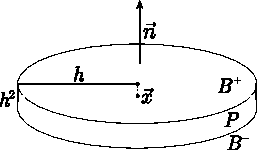
\includegraphics[width=0.6\textwidth]{images/sample.pdf}
% % \caption[caption za v kazalo]{Dolg caption pod sliko}
%   \caption[Primer vektorske slike.]{Primer vektorske slike z oznakami v enaki pisavi, kot jo
%      uporablja \LaTeX{}.  Narejena je s programom Inkscape, \LaTeX{} oznake so importane v
%      Inkscape iz pomožnega PDF.}
%   \label{fig:sample}
% \end{figure}
%
% \begin{figure}[h]
%   \centering
%   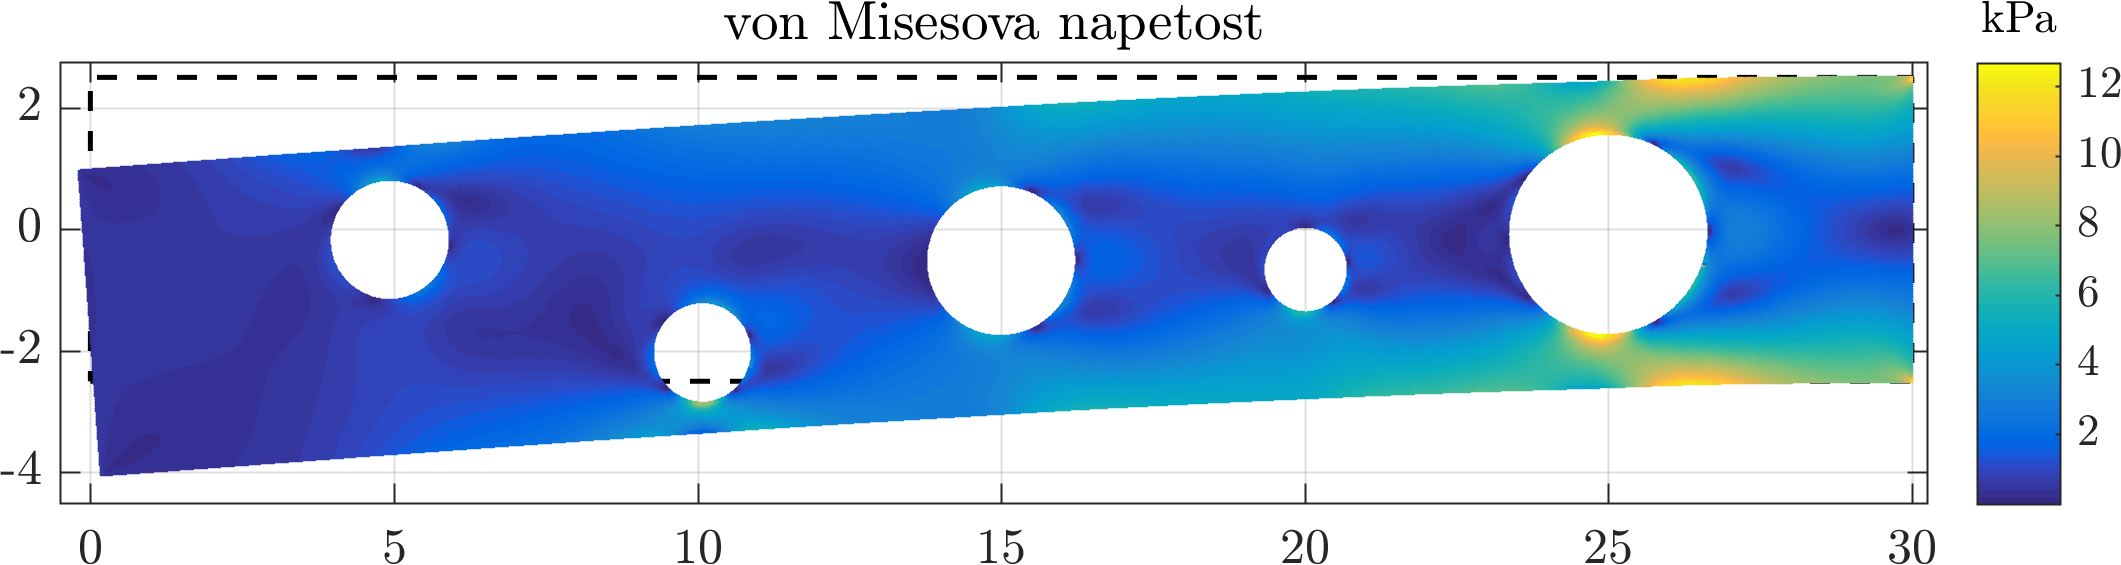
\includegraphics[width=0.8\textwidth]{images/image.png}
%   \caption[Primer bitne slike.]{Primer bitne slike, izvožene iz Matlaba. Poskrbite, da so slike v
%   dovolj visoki resoluciji in da ne vsebujejo prosojnih elementov (to zahteva PDF/A-1b format).}
%   \label{fig:image}
% \end{figure}
%
% \subsection{Kako narediti stvarno kazalo}
% Dodate ukaze \verb|\index{polje}| na besede, kjer je pojavijo, kot tukaj\index{tukaj}.
% Več o stvarnih kazalih je na voljo na \url{https://en.wikibooks.org/wiki/LaTeX/Indexing}.
%
% \subsection{Navajanje literature}
% Članke citiramo z uporabo \verb|\cite{label}|, \verb|\cite[text]{label}| ali pa več naenkrat s
% \verb|\cite\{label1, label2}|. Tudi tukaj predhodno besedo in citat povežemo z nedeljivim presledkom
% $\sim$. Na primer~\cite{chen2006meshless,liu2001point}, ali pa \cite{kibriya2007empirical}, ali pa
% \cite[str.\ 12]{trobec2015parallel}, \cite[enačba (2.3)]{pereira2016convergence}.
% Vnosi iz \verb|.bib| datoteke, ki niso citirani, se ne prikažejo v seznamu literature, zato jih
% tukaj citiram.~\cite{vene2000categorical}, \cite{gregoric2017stopniceni}, \cite{slak2015induktivni},
% \cite{nsphere}, \cite{kearsley1975linearly}, \cite{STtemplate}, \cite{NunbergerTand}, \cite{vanoosten2008realizability}.

\end{document}
